% Cole Nielsen niels538@umn.edu
% EE 2002 Spring 2015
% Formal Lab Report 3

%----------------------------------------------------------------------------------------
%	PACKAGES AND DOCUMENT CONFIGURATIONS
%----------------------------------------------------------------------------------------

\documentclass[12pt]{article}

\usepackage{circuitikz}
\usepackage{graphicx}
\usepackage{subcaption}
\usepackage[top=1in, bottom= 1in, left=1in, right= 1in]{geometry}
\setlength\parindent{0pt}
\usepackage{fancyhdr}
\pagestyle{fancy}
\usepackage{textcomp}
\usepackage{tikz}
\usepackage{siunitx}
\usepackage{placeins}
\usepackage{titlesec}
\usepackage{cancel} 
\usepackage{tikz}
\usetikzlibrary{shapes.geometric, arrows}
\tikzstyle{box} = [rectangle, rounded corners, minimum width = 3cm, minimum height = 1cm, text centered, draw = black]
\tikzstyle{arrow} = [thick,->,>=stealth]
\usepackage{placeins}

\usepackage{listings}
\usepackage{color}

\definecolor{dkgreen}{rgb}{0,0.6,0}
\definecolor{gray}{rgb}{0.5,0.5,0.5}
\definecolor{mauve}{rgb}{0.58,0,0.82}

\lstset{frame=tb,
  language=,
  aboveskip=3mm,
  belowskip=3mm,
  showstringspaces=false,
  columns=flexible,
  basicstyle={\small\ttfamily},
  numbers=none,
  numberstyle=\tiny\color{gray},
  keywordstyle=\color{blue},
  commentstyle=\color{dkgreen},
  stringstyle=\color{mauve},
  breaklines=true,
  breakatwhitespace=true,
  tabsize=3
}

%----------------------------------------------------------------------------------------
%	DOCUMENT INFORMATION
%----------------------------------------------------------------------------------------

\title{Lab 3 Report\\ \vspace{0.3 in} EE 4111}

\newcommand{\mymeter}[2]{   	% #1 = name , #2 = rotation angle
 \begin{scope}[transform shape,rotate=#2]
   \draw[thick] (#1)node(){$\mathbf V$} circle (11pt);
   \draw[rotate=45,-latex] (#1)  +(-17pt,0) --+(17pt,0);
 \end{scope}
}
\author{Cole \textsc{Nielsen}}
\date{Spring 2016}
\begin{document}
\maketitle 
\pagebreak
%---------------------------------------------------------------------------------------
%----------------------------------------------------------------------------------------
%	Introduction
%----------------------------------------------------------------------------------------
\section*{Spice File}
Below is the SPICE netlist file and the schematic of the compensated OP-AMP designed in this lab. The general netlist is listed only once to save space, any modifications made will be described in the according sections. The current source used in the compensation network was implemented as an ideal source as suggested by Prof. Higman.
\FloatBarrier
\begin{figure}[h!]
\begin{center}
 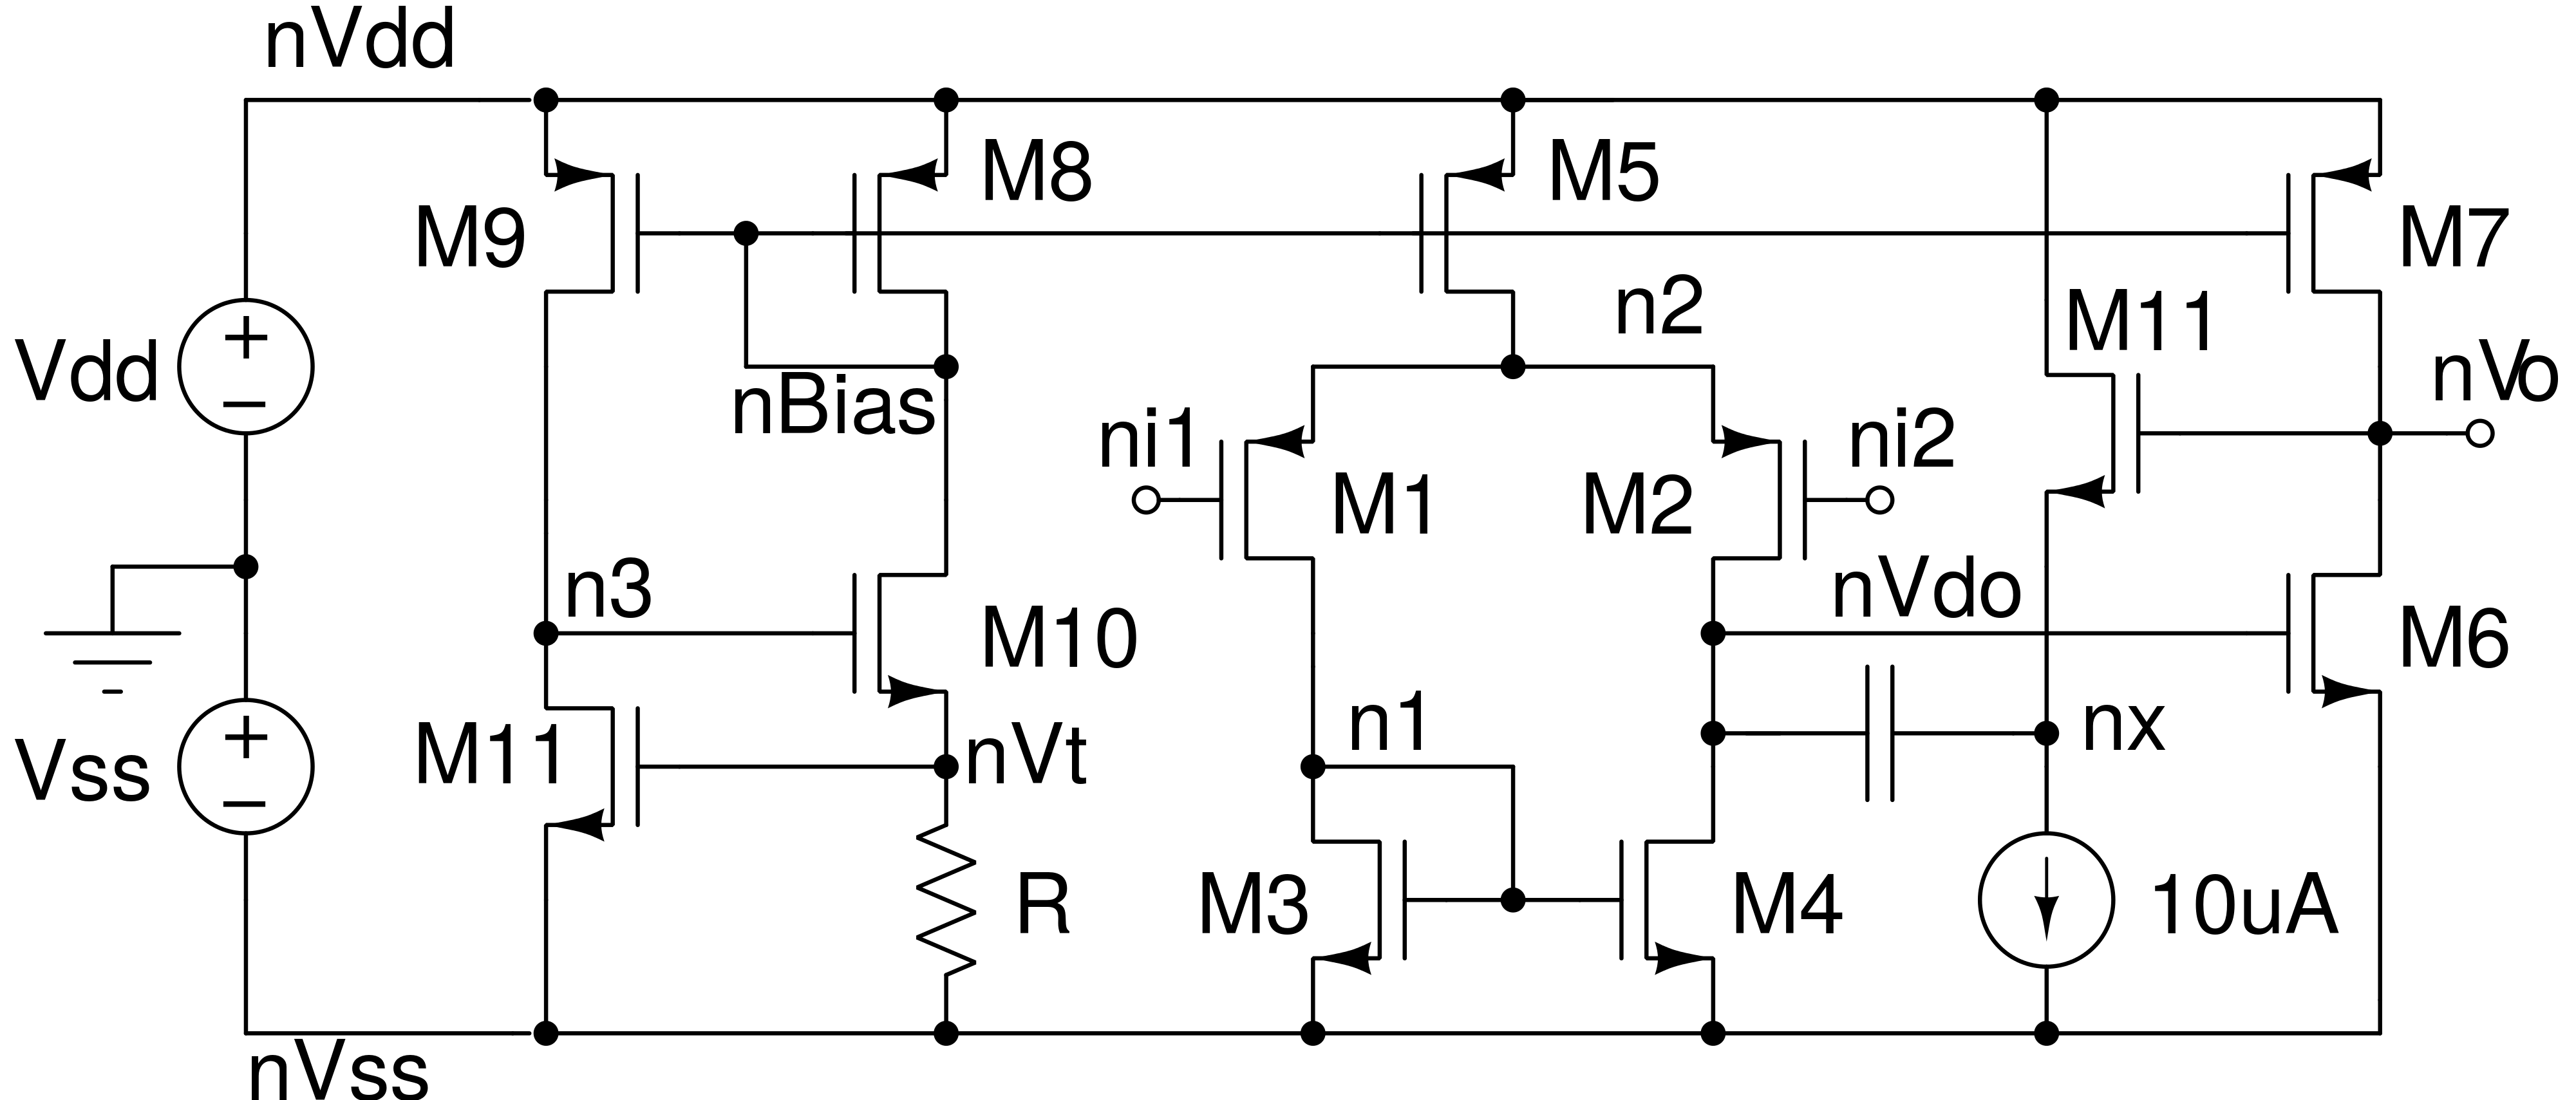
\includegraphics[scale=0.14]{./schem.png}
\end{center}
\end{figure}
\FloatBarrier
\begin{lstlisting}
TWO STAGE OPAMP
*******SIMULATION PARAMETERS*************
.OPTIONS LIST NODE POST
*.DC Vid -0.001 0.001 0.000001
.OP
*.TRAN 10ps 75n
.PRINT DC V(nvo) V(nvdo) V I1(M1) I1(M2) I1(M10) PAR('V(ni1)-V(ni2)')
*.PRINT DC V(n4) V(n5) V(n7) I1(M1) I1(M2) PAR('V(n1)-V(n2)') I(R2) I1(M6)
.AC DEC 30 1 1E9

.parameter Vid = 0
.parameter Vic = 0
.parameter Vios = -213.913u ***input offset
.parameter length = 0.25u

***********SUPPLIES*************
Vdd nvdd 0 DC 2V
Vss 0 nvss DC 2V
*Vi1 ni1 0 DC Vios	*for AC sweep/transient
Vi2 ni2 0 DC 0 AC 1 PULSE(0 1 25n 10p 10p 50n 1u)
*Ei1 ni1 0 VOL = 'Vios + Vic + Vid'  *used for DC sweep
*Ei2 ni2 0 VOL = 'Vic - Vid'

***********CURRENT REF**********
Rb nvt nvss 26000

M8 nbias nbias nvdd nvdd CMOSP W = 30u L = length
M9 n3 nbias nvdd nvdd CMOSP W = 16u L = length
M10 nbias n3 nvt nvss CMOSN W = 10u L = length
M11 n3 nvt nvss nvss CMOSN W = 10u L = length
*Mx D G S B CMOSx W = width L = length

************DIFF AMP*************
M1 n1 nvo n2 nvdd CMOSP W = 10u L = length
M2 nvdo ni2 n2 nvdd CMOSP W = 10u L = length 
M3 n1 n1 nvss nvss CMOSN W = 4u L = length
M4 nvdo n1 nvss nvss CMOSN W = 4u L = length
M5 n2 nbias nvdd nvdd CMOSP W = 16u L = length

*************STAGE 2*************

M6 nvo nvdo nvss nvss CMOSN W = 2.3u L = length
M7 nvo nbias nvdd nvdd CMOSP W =6u L = length
*Cl nvo 0 10p

***********COMPENSATION*************
*Cc nvdo nx 0.24pF
*M12 nvdd nvo nx nvss CMOSN W = 100u L = length
*Ibias nx nvss 10u

.MODEL CMOSN NMOS (
+LEVEL   = 49             acm     = 3              hdif    = 0.35e-6
+VERSION = 3.1            TNOM    = 27             TOX     = 5.7E-9
+XJ      = 1E-7           NCH     = 2.3549E17      VTH0    = 0.4365497
+K1      = 0.3915623      K2      = 0.0175145      K3      = 1E-3
+K3B     = 2.6588343      W0      = 1E-7           NLX     = 1.111465E-7
+DVT0W   = 0              DVT1W   = 0              DVT2W   = 0
+DVT0    = -0.0408321     DVT1    = 0.0746768      DVT2    = 0.307109
+U0      = 407.1177485    UA      = 9.442714E-11   UB      = 1.092986E-18
+UC      = 1.63196E-11    VSAT    = 1.365087E5     A0      = 1.3189329
+AGS     = 0.2711719      B0      = 3.291713E-8    B1      = -1E-7
+KETA    = 4.645753E-3    A1      = 0              A2      = 1
+RDSW    = 439.9558234    PRWG    = 0.0345487      PRWB    = -0.0441065
+WR      = 1              WINT    = 1.645705E-9    LINT    = 1.116516E-9
+XL      = 3E-8           XW      = 0              DWG     = -1.494138E-9
+DWB     = 1.459097E-8    VOFF    = -0.1026054     NFACTOR = 0.1344887
+CIT     = 0              CDSC    = 1.527511E-3    CDSCD   = 0
+CDSCB   = 0              ETA0    = 1.930311E-3    ETAB    = 2.946158E-4
+DSUB    = 0.0214865      PCLM    = 1.3387947      PDIBLC1 = 0.480652
+PDIBLC2 = 9.034986E-3    PDIBLCB = -1E-3          DROUT   = 0.5593223
+PSCBE1  = 9.843289E9     PSCBE2  = 2.10878E-9     PVAG    = 1.0033136
+DELTA   = 0.01           MOBMOD  = 1              PRT     = 0
+UTE     = -1.5           KT1     = -0.11          KT1L    = 0
+KT2     = 0.022          UA1     = 4.31E-9        UB1     = -7.61E-18
+UC1     = -5.6E-11       AT      = 3.3E4          WL      = 0
+WLN     = 1              WW      = -1.22182E-16   WWN     = 1.2127
+WWL     = 0              LL      = 0              LLN     = 1
+LW      = 0              LWN     = 1              LWL     = 0
+CAPMOD  = 2              XPART   = 0.4            CGDO    = 3.11E-10
+CGSO    = 3.11E-10       CGBO    = 1E-11          CJ      = 1.758521E-3
+PB      = 0.99           MJ      = 0.457547       CJSW    = 4.085057E-10
+PBSW    = 0.8507757      MJSW    = 0.3374073      PVTH0   = 7.147521E-5
+PRDSW   = -67.2161633    PK2     = -1.344599E-3   WKETA   = 3.035972E-3
+LKETA   = -9.0406E-3     LAGS    = -0.3012         )
*
.MODEL CMOSP PMOS (
+LEVEL   = 49             acm     = 3              hdif    = 0.35e-6
+VERSION = 3.1            TNOM    = 27             TOX     = 5.7E-9
+XJ      = 1E-7           NCH     = 4.1589E17      VTH0    = -0.6586391
+K1      = 0.5199897      K2      = 0.0357513      K3      = 0
+K3B     = 15.5613889     W0      = 1E-6           NLX     = 1E-9
+DVT0W   = 0              DVT1W   = 0              DVT2W   = 0
+DVT0    = 2.6100181      DVT1    = 0.4363142      DVT2    = -0.042436
+U0      = 196.024903     UA      = 2.767112E-9    UB      = 1.90709E-18
+UC      = 6.166867E-11   VSAT    = 1.975064E5     A0      = 0.2398712
+AGS     = 0.0943234      B0      = 3.21184E-6     B1      = 5E-6
+KETA    = 0.0312217      A1      = 0              A2      = 1
+RDSW    = 997.072701     PRWG    = -0.1916111     PRWB    = -0.495
+WR      = 1              WINT    = 2.527293E-9    LINT    = 1.254514E-8
+XL      = 3E-8           XW      = 0              DWG     = -3.253948E-8
+DWB     = 4.92072E-8     VOFF    = -0.15          NFACTOR = 1.5460516
+CIT     = 0              CDSC    = 1.413317E-4    CDSCD   = 0
+CDSCB   = 0              ETA0    = 0.7241245      ETAB    = -0.240523
+DSUB    = 1.0813613      PCLM    = 2.0772083      PDIBLC1 = 4.31459E-4
+PDIBLC2 = 0.0252121      PDIBLCB = -9.960722E-4   DROUT   = 0.0432774
+PSCBE1  = 3.191047E10    PSCBE2  = 1.323218E-8    PVAG    = 0.0420525
+DELTA   = 0.01           MOBMOD  = 1              PRT     = 0
+UTE     = -1.5           KT1     = -0.11          KT1L    = 0
+KT2     = 0.022          UA1     = 4.31E-9        UB1     = -7.61E-18
+UC1     = -5.6E-11       AT      = 3.3E4          WL      = 0
+WLN     = 1              WW      = 0              WWN     = 1
+WWL     = 0              LL      = 0              LLN     = 1
+LW      = 0              LWN     = 1              LWL     = 0
+CAPMOD  = 2              XPART   = 0.4            CGDO    = 2.68E-10
+CGSO    = 2.68E-10       CGBO    = 1E-11          CJ      = 1.902493E-3
+PB      = 0.9810285      MJ      = 0.4644362      CJSW    = 3.142741E-10
+PBSW    = 0.9048624      MJSW    = 0.3304452      PVTH0   = 4.952976E-3
+PRDSW   = 29.8169373     PK2     = 3.383373E-3    WKETA   = -7.913501E-3
+LKETA   = -0.0208318      )
*
.end
\end{lstlisting}
\section{OP-AMP Non-Compensated Response}
The first objective of this lab was to determine the frequency response of the OP-AMP designed in Lab 2 without any compensation. This would be the netlist listed above with the compensation section commented out. The frequency response was analyzed in terms of CMRR, which is given as:
\begin{equation}
\textnormal{CMRR}(\omega) = \frac{A_{d}(\omega)}{A_{c}(\omega)}
\end{equation}
It is simply the ratio of differential gain to common mode gain. This was calculated as a function of frequency by finding $A_d$ and $A_c$ separately in SPICE. Note: the the input offset voltage was compensated with a DC source before hand to eliminate errors due to DC offset. To find $A_d$, one input was grounded and the other was driven with a AC source in a AC simulation, yielding a waveform for $A_d(\omega)$. $A_c(\omega)$ was found by connecting both the inputs of the OP-AMP together to a AC source and running the same AC simulation. $CMRR(\omega)$ was then calculated in COSMOSCOPE by dividing $A_d(\omega)$ by $A_c(\omega)$ and plotting the result for the output node, this is shown below. The pole was found at 10.055 Hz.
\FloatBarrier
\begin{figure}[h!]
\begin{center}
 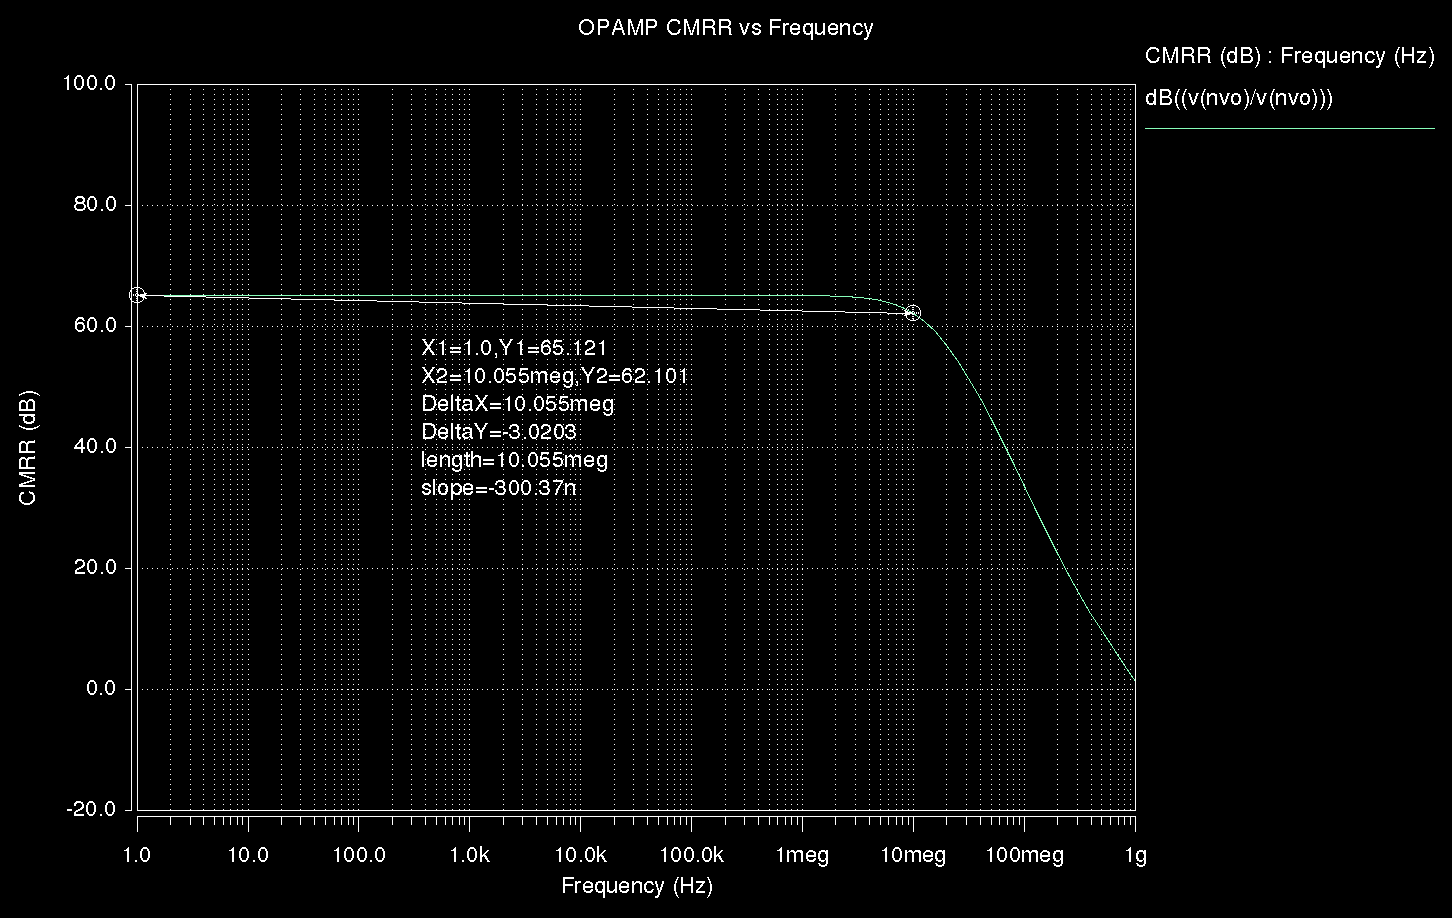
\includegraphics[scale=0.3]{./cmrr.png}
\end{center}
\end{figure}
\FloatBarrier
Below is a plot that shows the seperate graphs for differential gain, common mode gain and the combined CMRR. Notice the differential gain nominally being around 60dB and the common mode gain being nominally around -10dB. Interestingly the common mode gain increases approaching 200 MHz and then later deceases after 200 MHz.
\FloatBarrier
\begin{figure}[h!]
\begin{center}
 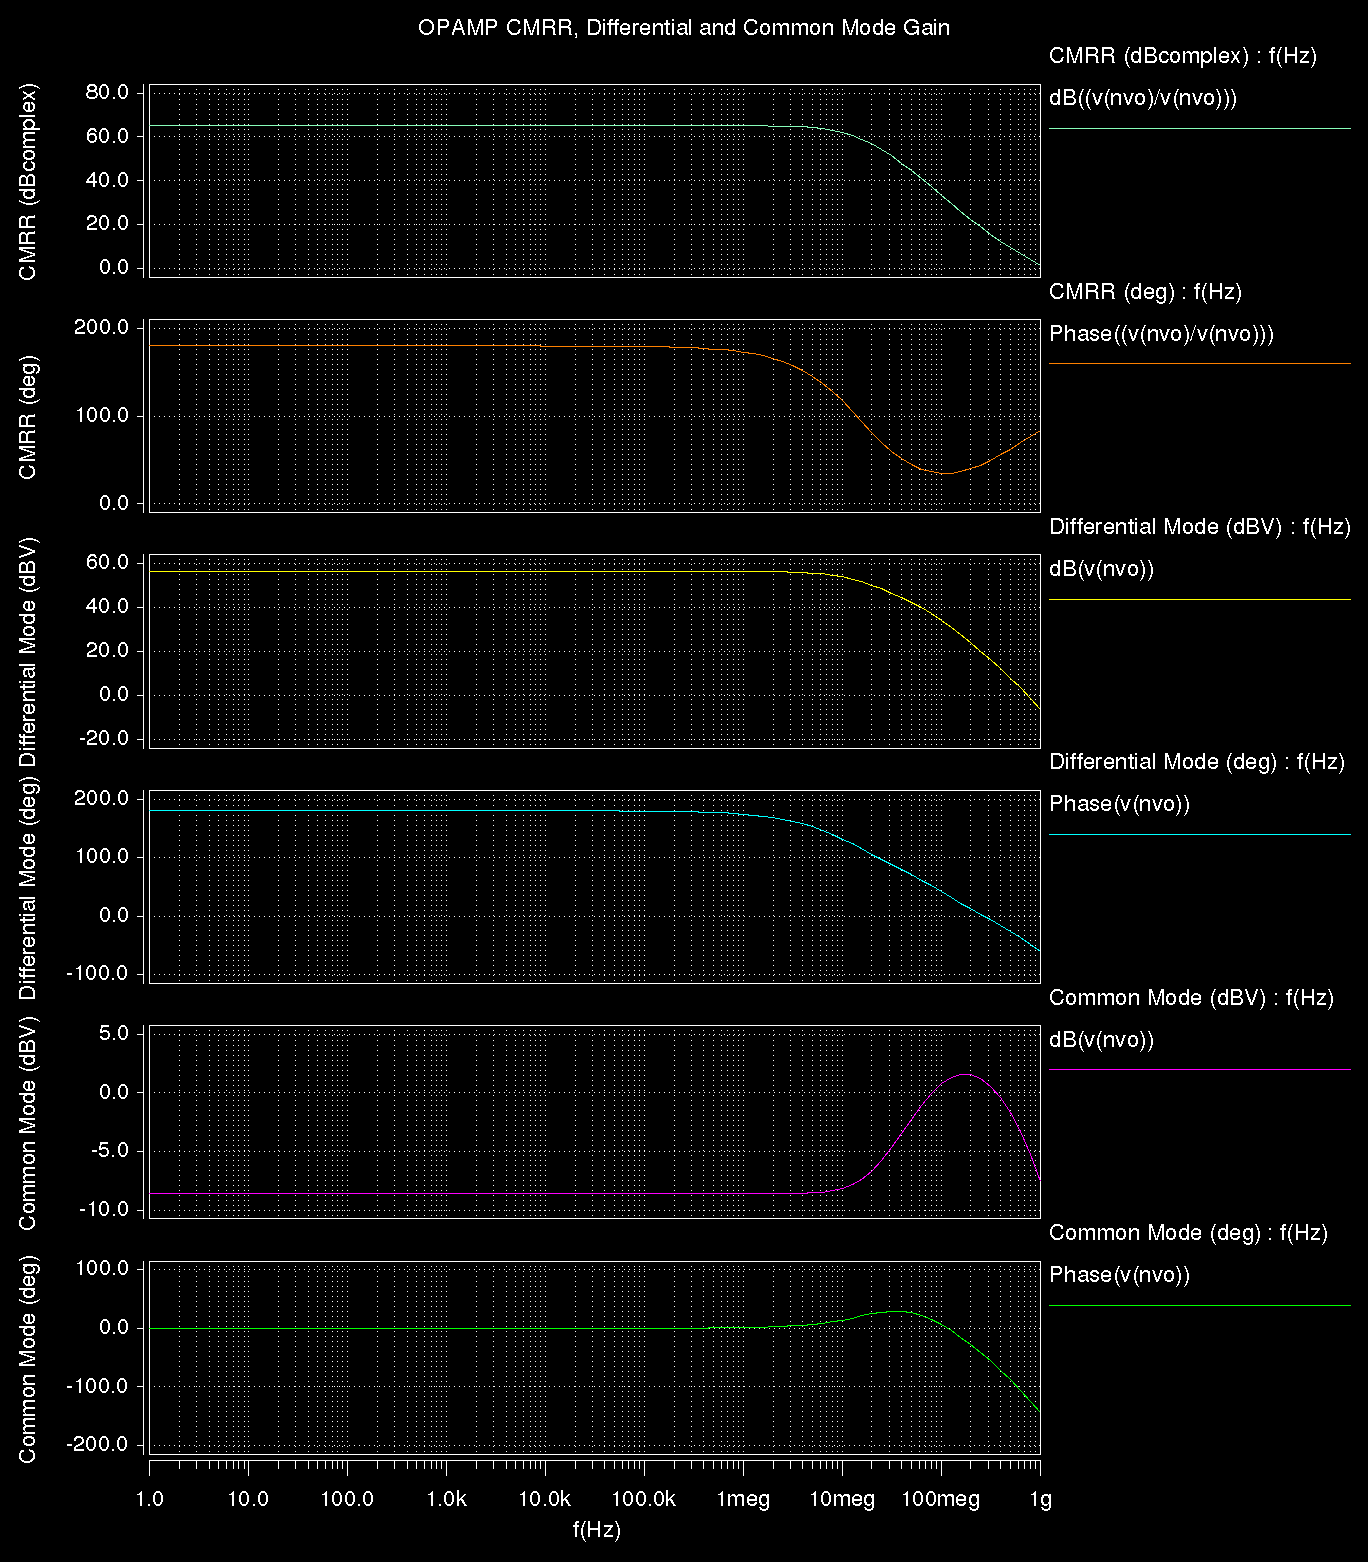
\includegraphics[scale=0.3]{./cmrrfull.png}
\end{center}
\end{figure}
\FloatBarrier
A second analysis was performed in this part, which was determining the effect of the signal source resistance on the input pole location. This was done by simply adding a resistor between the OP-AMP input and the input voltage source, and then simulating the AC response for different R values. Below is the plot showing this effect (measured at the output node of the input stage), it can be seen that the pole location decreases in frequency with $R_s$ value, which makes sense as cutoff frequency $f_c = \frac{1}{2\pi RC}$, where $R\rightarrow\infty$ results in $f\rightarrow 0$. The location of the pole was not changed much by input resistance until approximately 100k$\Omega$ of source resistance was added, which dropped the pole by approximately 2.4 MHz from 10 MHZ. Any resistances above 100k$\Omega$ severely decreased the pole location, which would likely hinder designs requiring high frequency operation. The take away of this is to minimize the source resistance going to the input of an OP-AMP, especially in microelectronic circuits like this one.
\FloatBarrier
\begin{figure}[h!]
\begin{center}
 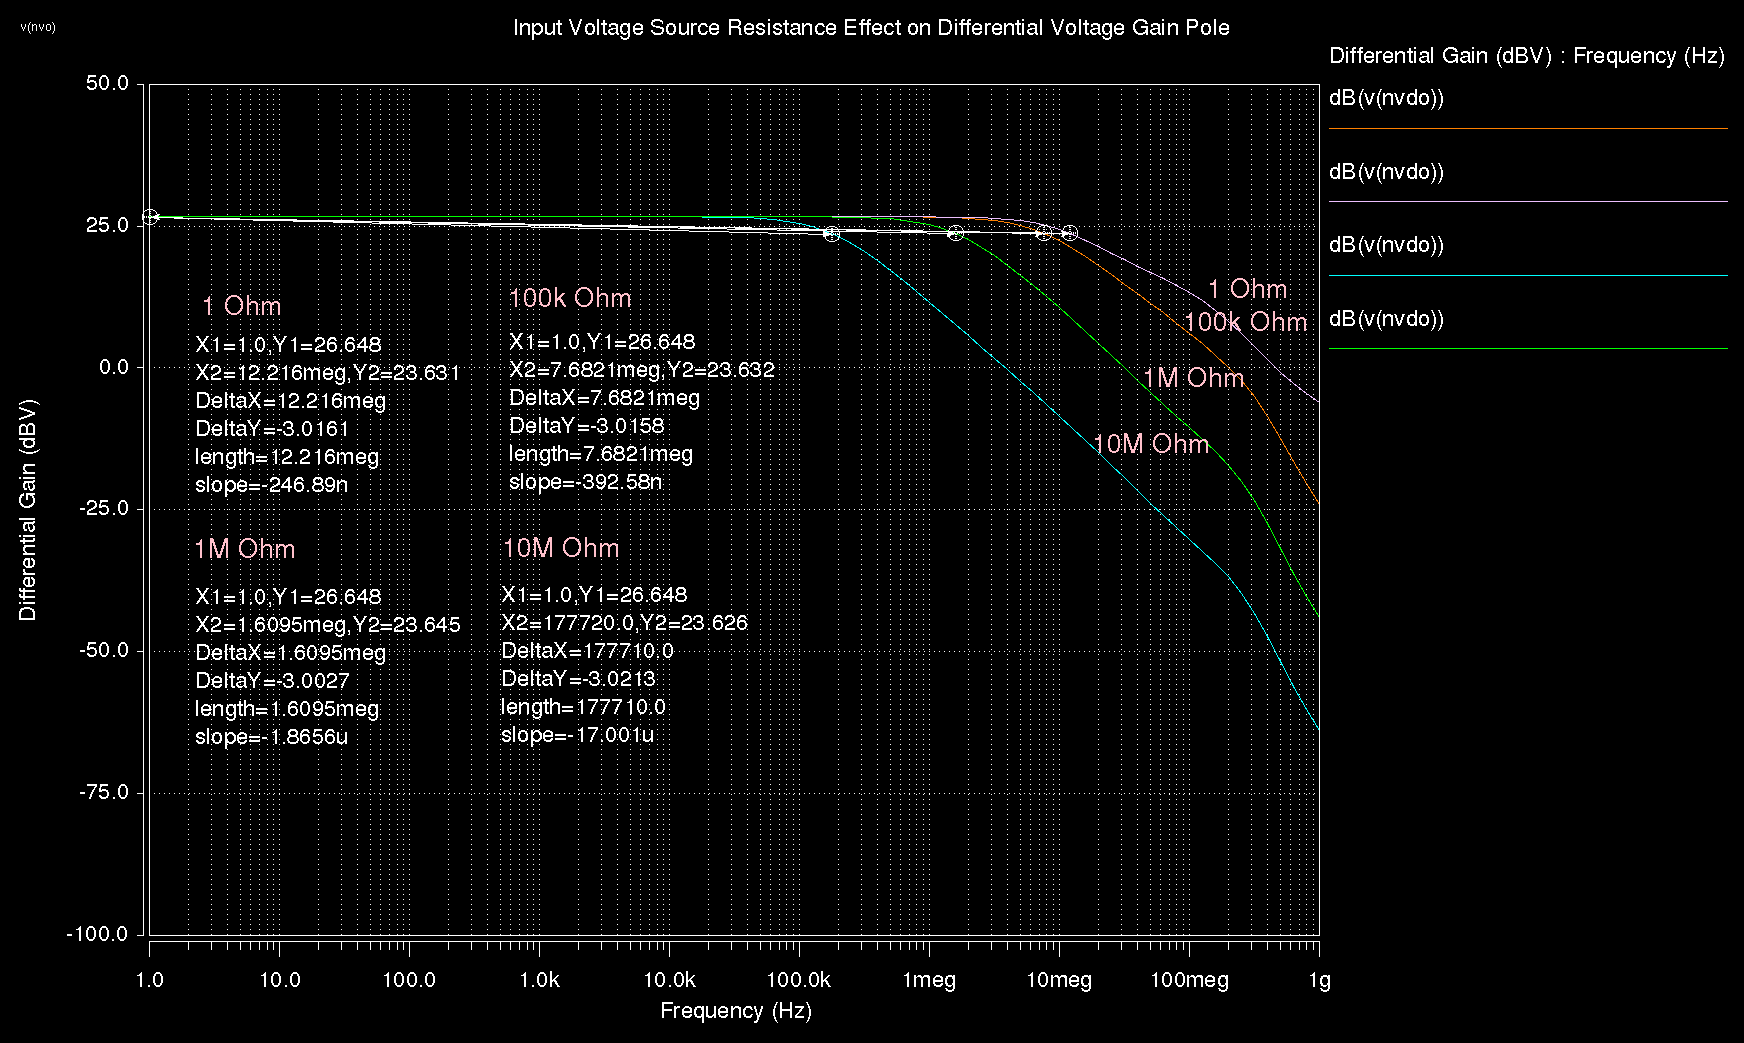
\includegraphics[scale=0.25]{./resistance.png}
\end{center}
\end{figure}
\FloatBarrier
\section{Implementation of Improved}
The second task of the lab was to implement an improved compensation topology in the OP-AMP, with a 60$ ^\circ$ phase margin afforded in doing so. The compensation method shown in figure 9.21 of Gray and Meyer was used in this implementation:
\FloatBarrier
\begin{figure}[h!]
\begin{center}
 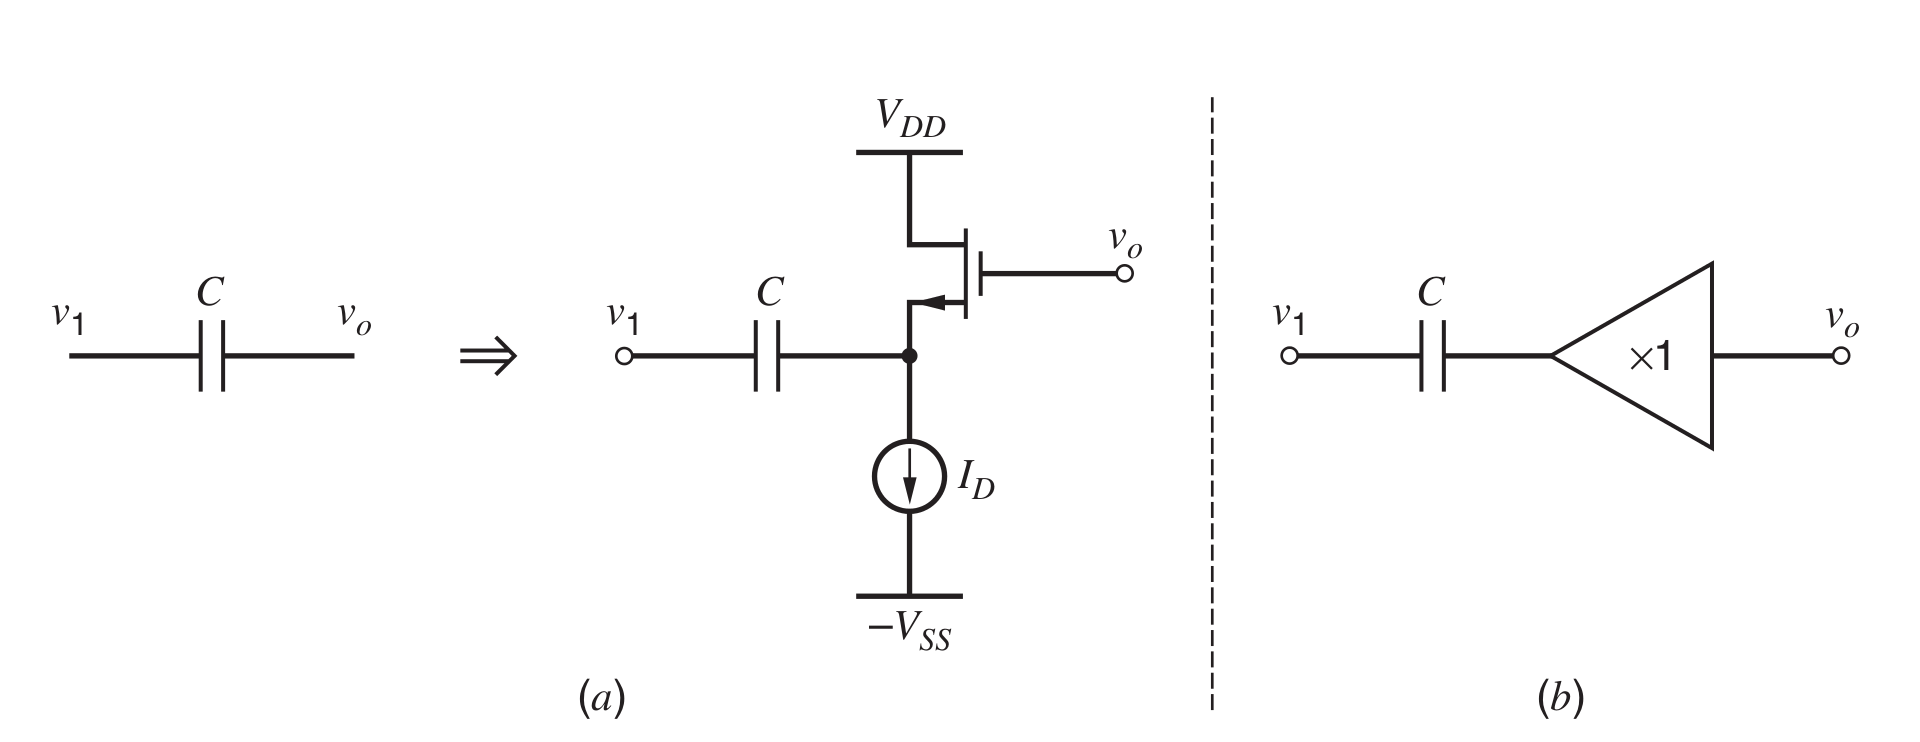
\includegraphics[scale=0.2]{./comp.png}
\end{center}
\end{figure}
\FloatBarrier
This compensation takes the feedback capacitor used originally between the first and second stage output, and replaces it with a buffer that sends feedback from the second stage output node through a compensation capacitor to the first stage output node. The buffer is implemented as a source follower built with a NMOS transistor and a current source. Signal gain for a source folower is given by:
\begin{equation}
A_v = \frac{1}{1+\frac{1}{g_m r_o}}
\end{equation}
Where $g_m r_o$ is the intrinsic gain $A_i$ of the transistor. If $A_i$ is maximized, the voltage gain will be very close to 1, which makes it a good buffer. $g_m r_o$ is calculated as:
\begin{equation}
A_i = g_m r_o = \frac{V_a}{i_d}\sqrt{2 i_d \mu_n C_{ox}\left(\frac{W}{L}\right)} = V_a \sqrt{\frac{2 \mu_n C_{ox}\left(\frac{W}{L}\right)}{i_d}}
\end{equation}
Therefore, using a large $\left(\frac{W}{L}\right)$ value and a small $i_d$ will yield a high $A_i$, which will in turn make a good buffer. Values used to achieve a well functioning buffer were $\left(\frac{W}{L}\right)$ = 400 and $i_d$ = 10 $\mu$A. C value sizing was done by testing several capacitor values until an acceptable response was observed. It was expected that the capacitor size would shrink in size compared to the original compensation capacitor C, so 1pF was tested as the initial compensation capacitor value. The pole location for that value was low enough to provide excess ($>$ 60$ ^\circ$) of phase margin. In order to maximize bandwith (by sacrificing phase margin), the capacitor value was then decreased to 0.1pF, which proved provided too little phase margin. Finally, 0.2 pF was tested, yielded approximately 45$ ^\circ$ of phase margin, which was close but still acceptable. More attempts lead to 0.24pF as the ideal C value, giving just 60$ ^\circ$ of phase margin (a phase of -119.62 for 0dB gain at 127.7 MHz). Below is a plot of the frequency response in differential mode of the compensated amplifier. The total bandwidth was found to be 127.7 MHz. Notice how visible the two pole locations are based on the the phase Bode plot (the two seperate regions where the phase drops).
\FloatBarrier
\begin{figure}[h!]
\begin{center}
 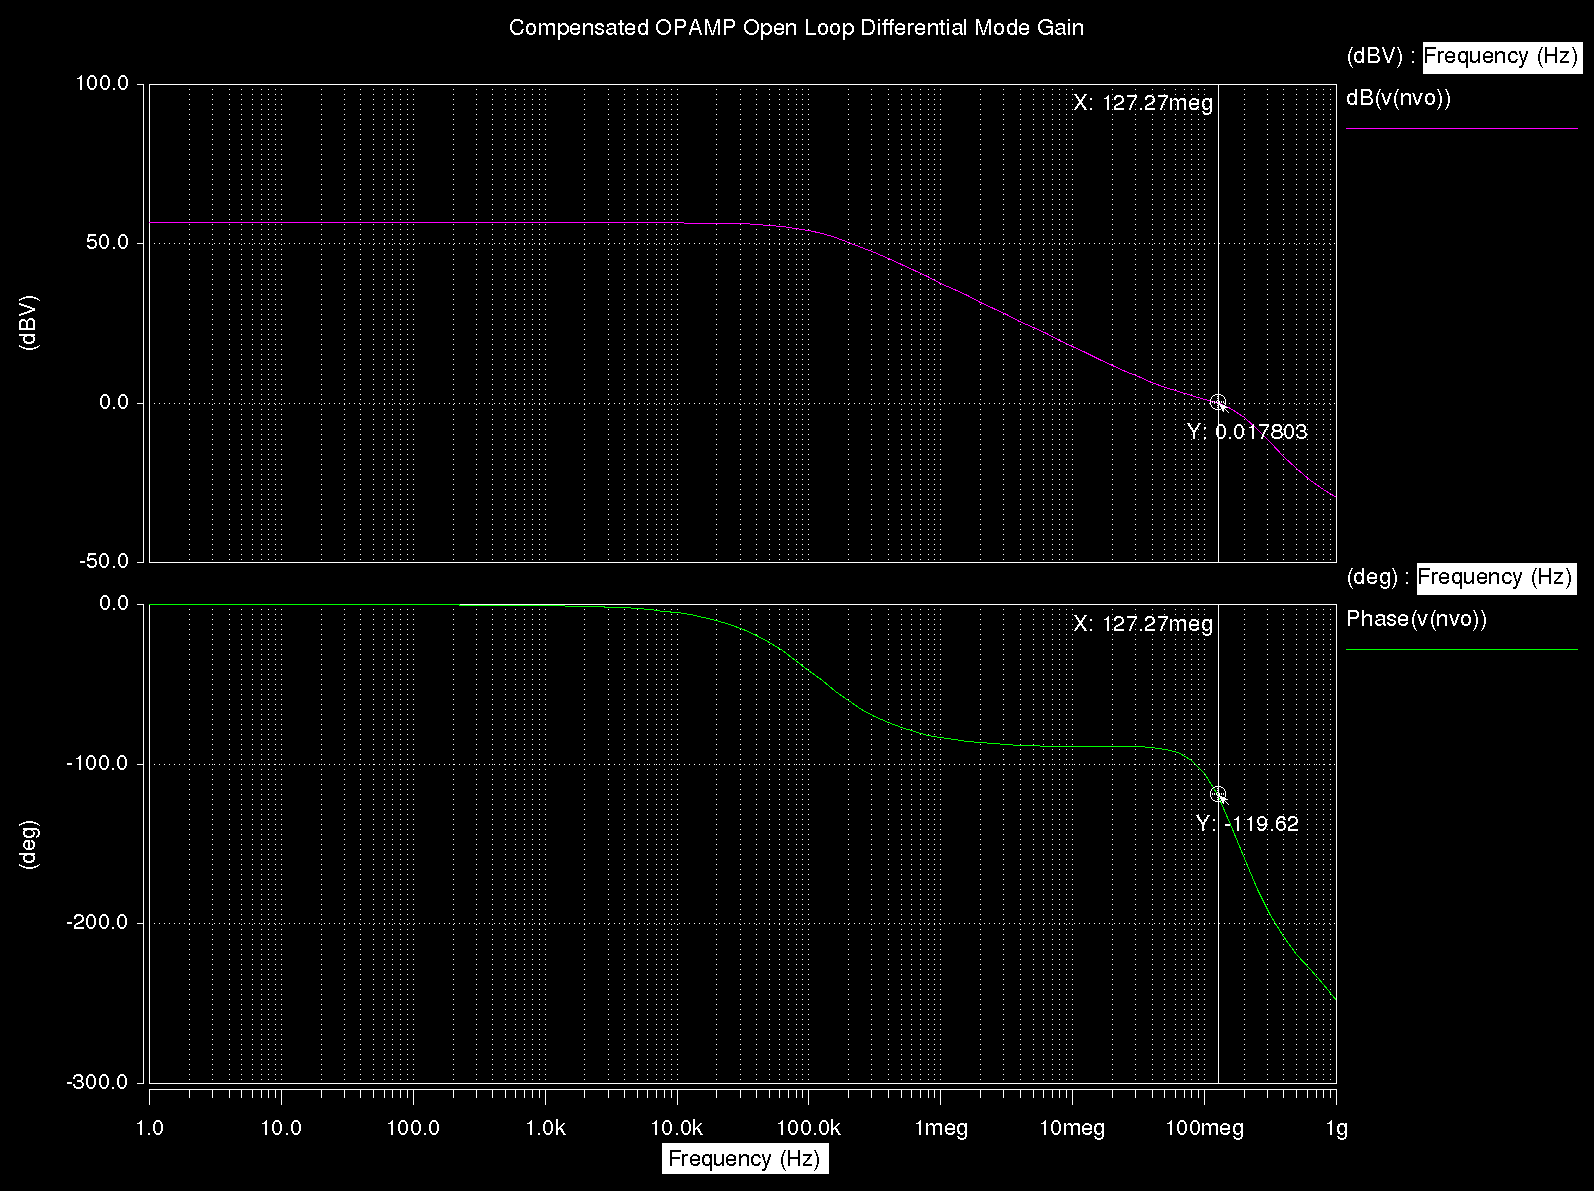
\includegraphics[scale=0.27]{./compensated.png}
\end{center}
\end{figure}
\FloatBarrier

\section{Compensated CMRR}
Using the same methods as the first section, the CMRR($\omega$) plot was found for the now compensated OP-AMP. Find the plot on the following page. The CMRR is of similar response compared to the original, however the pole has decreased slightly to 8.887 MHz from approximately 10 MHz. This drop in bandwidth is a acceptable loss when viewed from the standpoint of stability gained in the process, making the OP-AMP far more useful and reliable in the long run.
\FloatBarrier
\begin{figure}[h!]
\begin{center}
 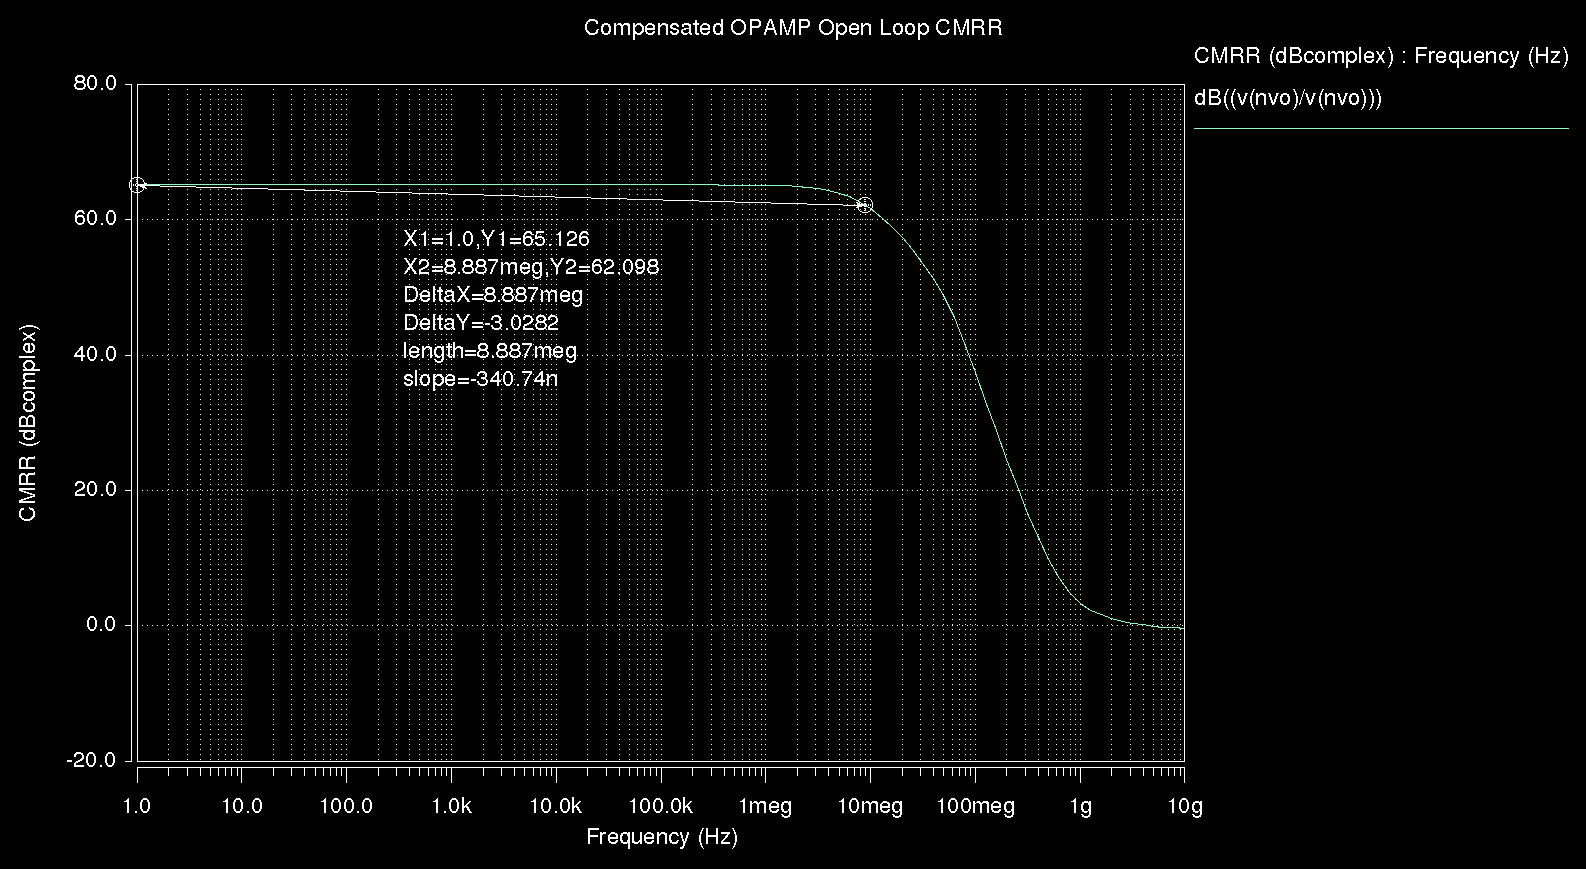
\includegraphics[scale=0.27]{./compcmrr.png}
\end{center}
\end{figure}
\FloatBarrier

\section{Unity Gain Follower Stability}
For this part, the objective was to find the stability of the OP-AMP in a unity-gain follower configuration. This is done by connecting the output (assuming it is non-inverting) to the inverting input of the OP-AMP, and then driving the other input with a signal source. Stability can easily be analyzed in two ways, with a frequency sweep, where unstable frequencies are where the response blows up, or by driving the input with a step that has essentially instant rise time. The step function acts like an extremely high frequncy excitation for the OP-AMP, so if it is unstable, oscillation is expected and should be observed in a transient simulation.
\subsection*{AC Sweep Stability Analysis}
A voltage source was connected to the input of the OP-AMP in the SPICE file, and a AC simulation was performed by exciting the input volage source. Below is the plot for frequency response $|H(\omega)|$ of the closed loop unity gain amplifier. It can be noted that the gain is 1 until close to the pole, where some gain peaking is observed of a few decibels, however the system remains stable because either the phase margin is always high enough (system is not in positive feedback), or the gain is sufficiently low ($<$1) at the points where the OP-AMP is in positive feedback (-180$ ^\circ$ phase). The implication of the gain peaking is that there will be slight gain for sinusoids in that frequency, or a decaying sinusoid will occur with a stimuli in that range. Stable oscillation will not occur, however, because the Barkhausen Criteria are not satisfied for any frequency for this OP-AMP. The Barkhausen criteria specifies the phase margin must strictly be 0$ ^\circ$ and the gain 1 to oscillate stably at some point (not observed in the simulation data). This is evident because the gain is -7 dB at 0 phase margin.
\begin{figure}[h!] 
\begin{center}
 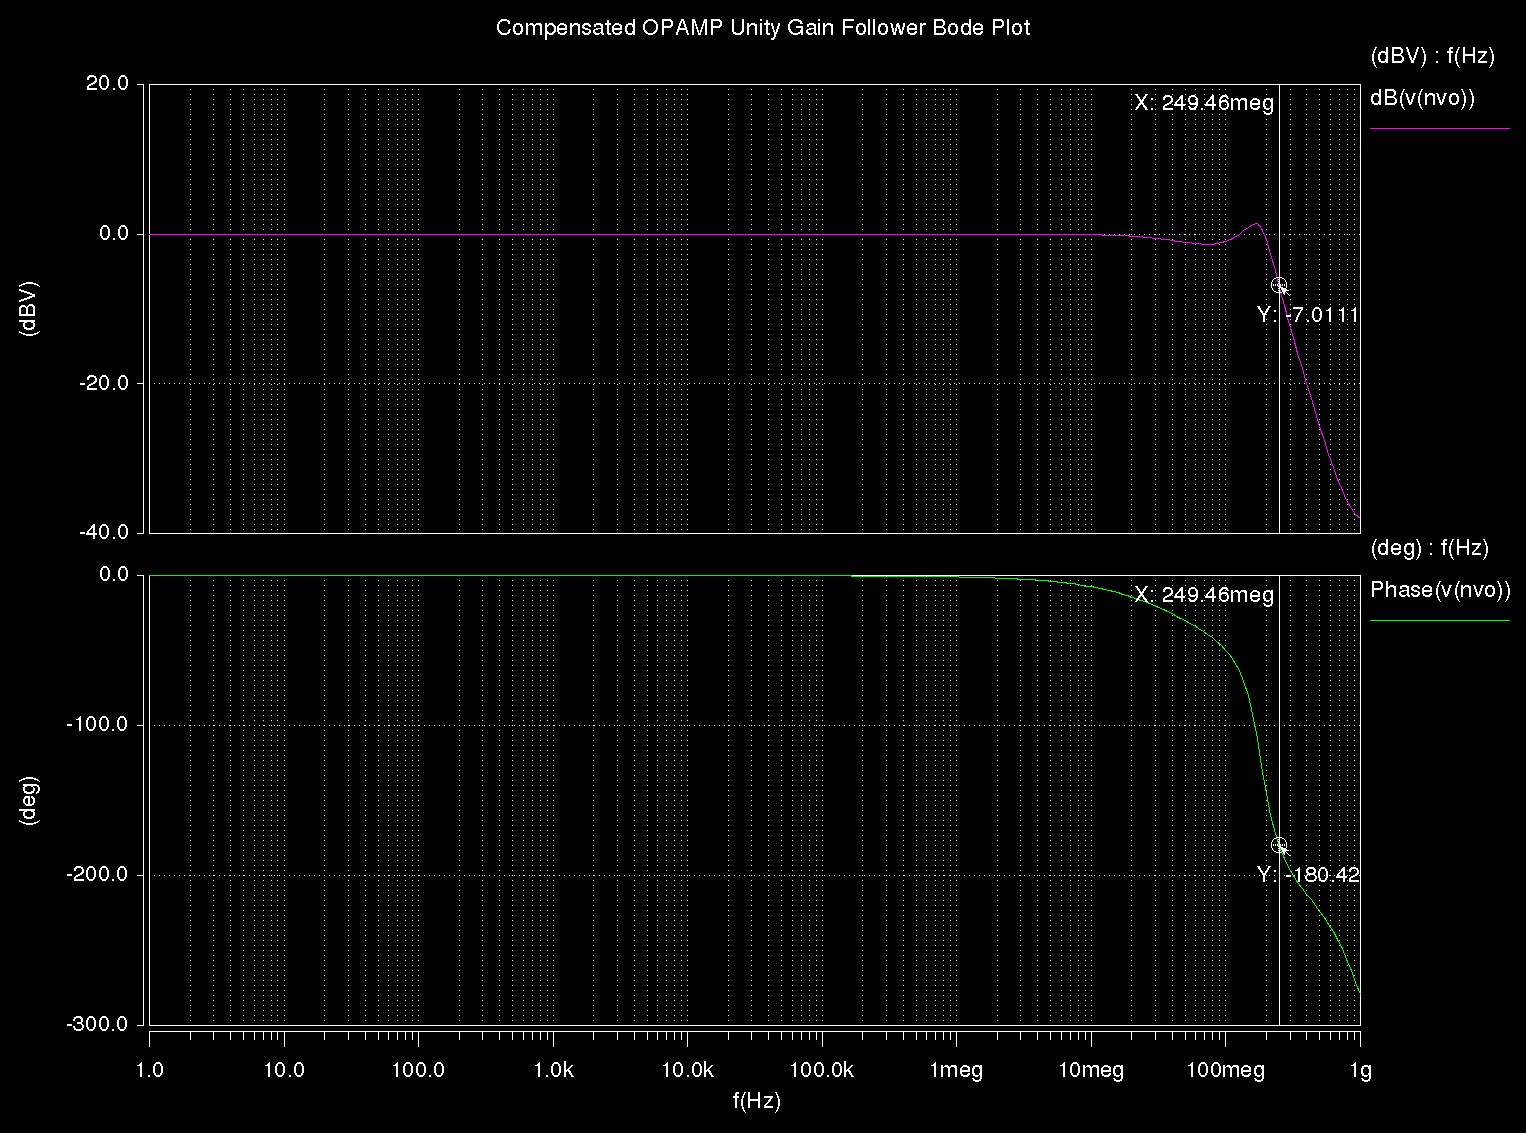
\includegraphics[scale=0.28]{./follower.png}
\end{center}
\end{figure}
\FloatBarrier
\subsection*{Step Transient Response Stability Analysis}
A DC source generating a step stimuli was connected to the input of the opamp and a transient simulation was performed to see the output response stability. Below is the output results for this simulation. It can be seen that for rising edges, the opamp behaves stably, however for a step with a falling edge, decaying oscillation is observed. The difference in stability for rising and falling edges is possible due to different effective capacitances caused by the input voltage level (capacitance tends to rise slightly with gate voltage), which may alter the stability. Also, the topology used is able to discharge the compensation capacitance faster than it can be charged, so it should be expected that the output will fall faster on a falling step, stimulating the system with higher frequency and inducing more oscillations. Nonetheless the response observed is still stable as the oscillations were decaying, showing the OP-AMP is effectively compensated, however perhaps not ideally so. It should also be noted that the rate of charging limit for the OP-AMP limits the slew rate (seen for the rising step). This slew rate limit is defined by the bias current of the differential input stage and the compensation capacitor value.
\begin{figure}[h!] 
\begin{center}
 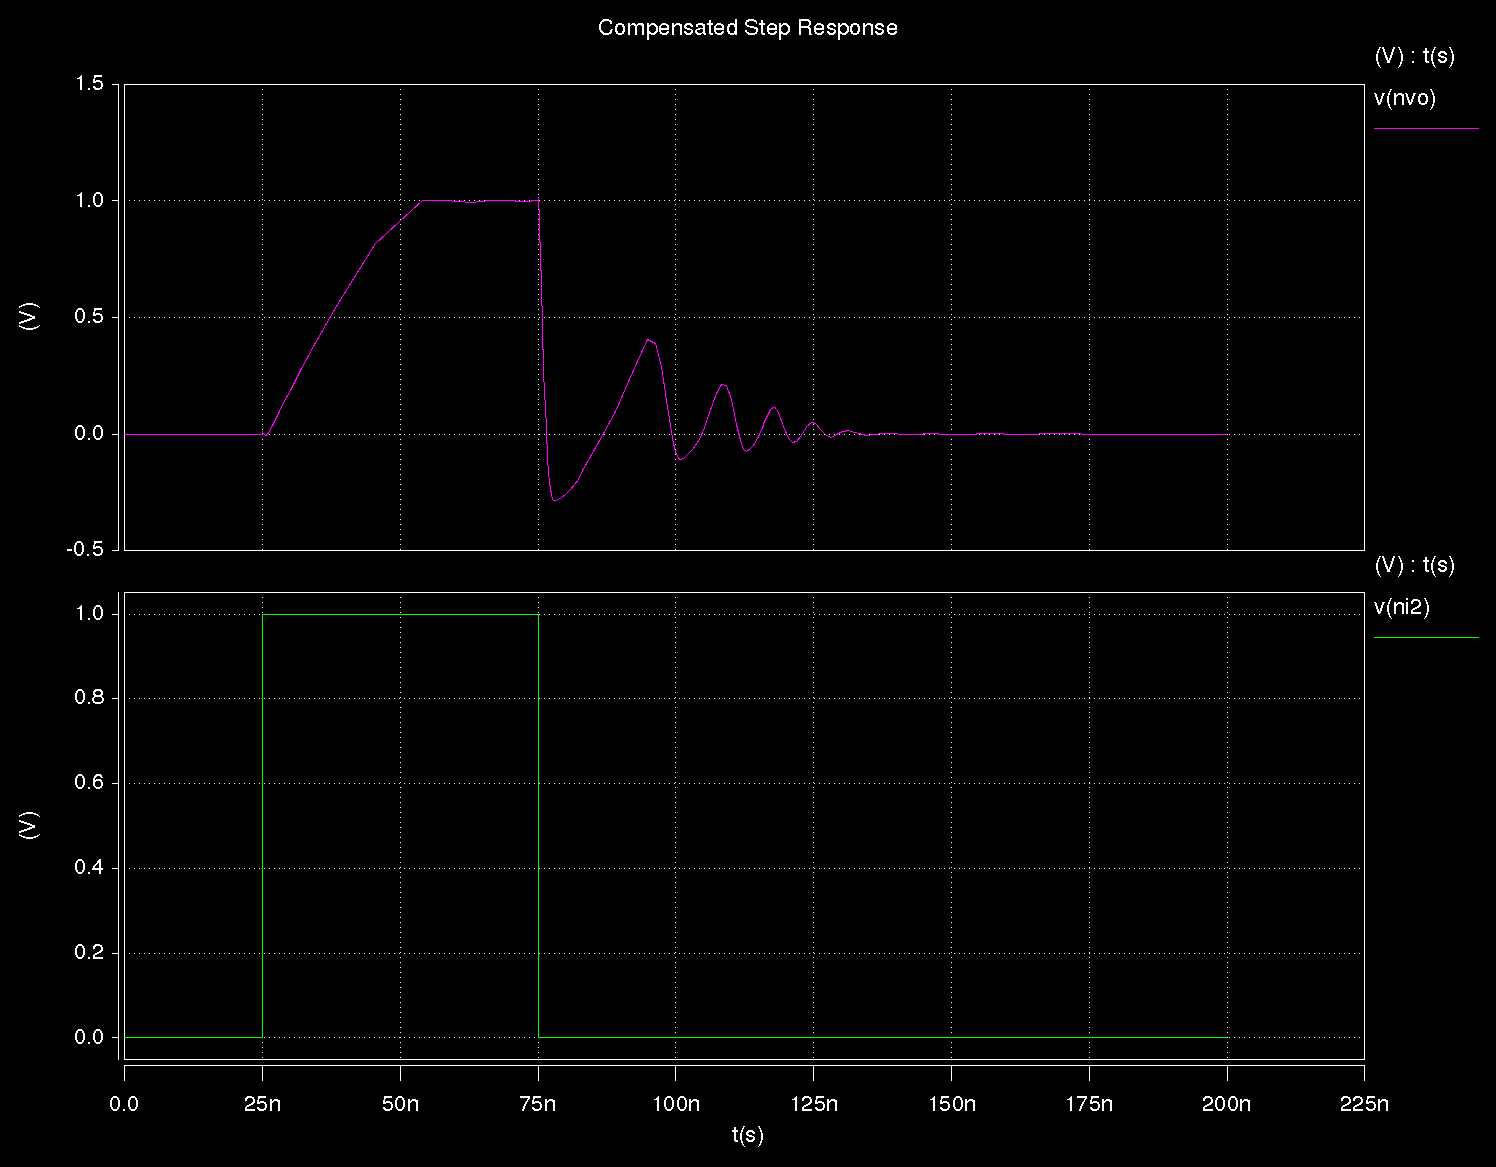
\includegraphics[scale=0.3]{./steppn.png}
\end{center}
\end{figure}
\FloatBarrier
\subsection*{Capacitive Loading and Stability}
For this part, several capacitive loads in the range of 2-10pF were attached to the output of the OP-AMP to observe the effect of capacitve loading on stability by performing an AC sweep. This was done because in CMOS microelectronics, loads are generally capactive, so it is important to understand the effect of capacitive loading on OP-AMP behavior. The plot on the following page demonstrates the effect of this loading for 10pF, 6pF and 2pF. It was generally seen that load capacitance decreased the pole frequency of the amplifier, decreasing with increasing capacitance values. The consequence of this is that the stability of the OP-AMP increases with capacitive loads, as evident by the gain at the -180$^\circ$ phase point decreases continually with load, going from -7dB with no load to -46.775dB at 10pF of loading (find plots Bode plots for individual capacitance values on the following pages). Practically this means that OP-AMPs in real circuits, where they are loaded, will be more stable than they are free-running, however they will have lower bandwidth then for when they are alone.
\FloatBarrier
\begin{figure}[h!] 
\begin{center}
 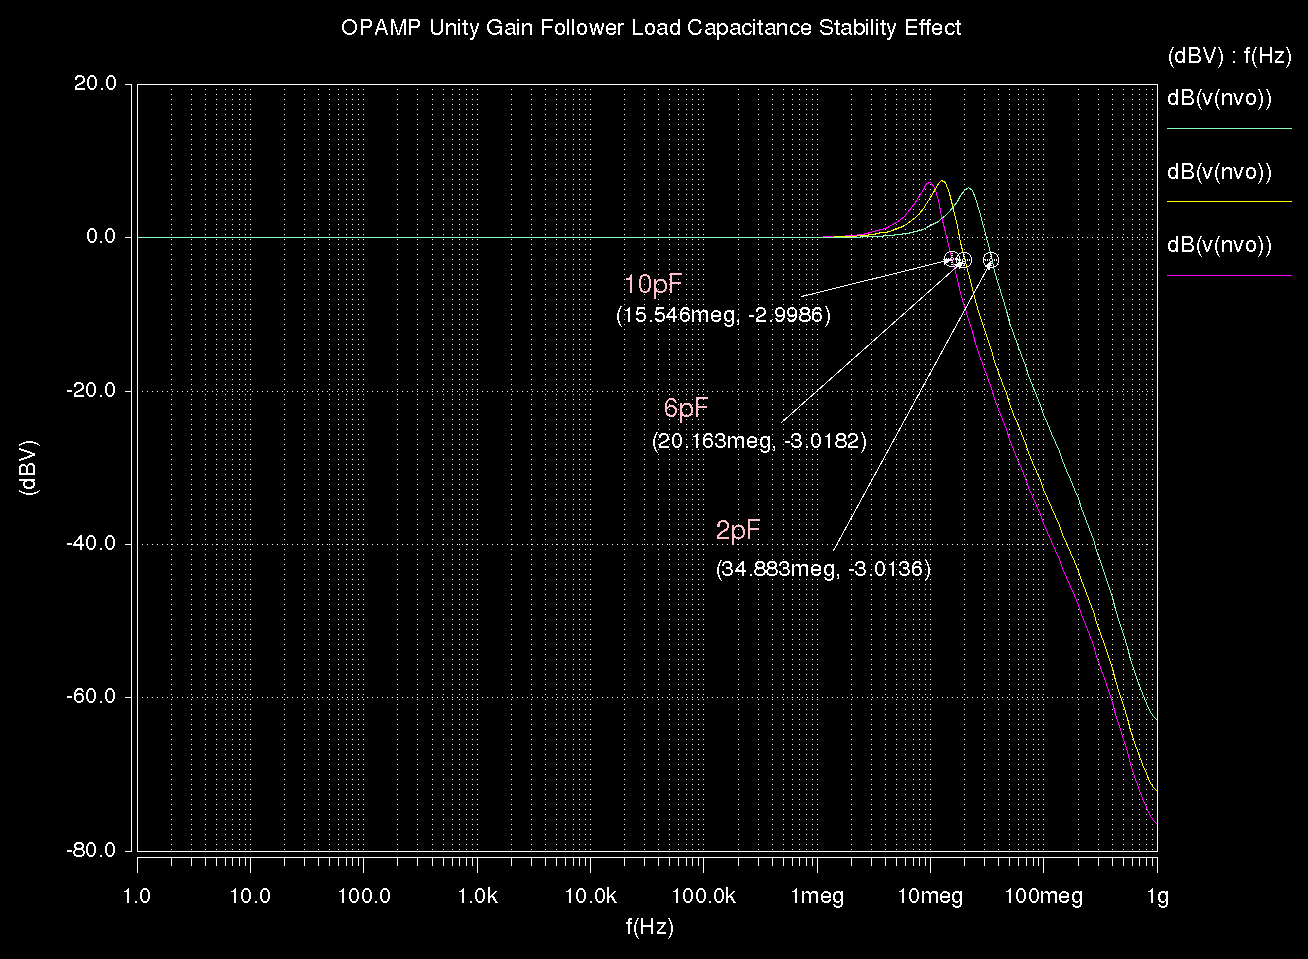
\includegraphics[scale=0.35]{./cap.png}
\end{center}
\end{figure}
\begin{figure}[h!] 
\begin{center}
 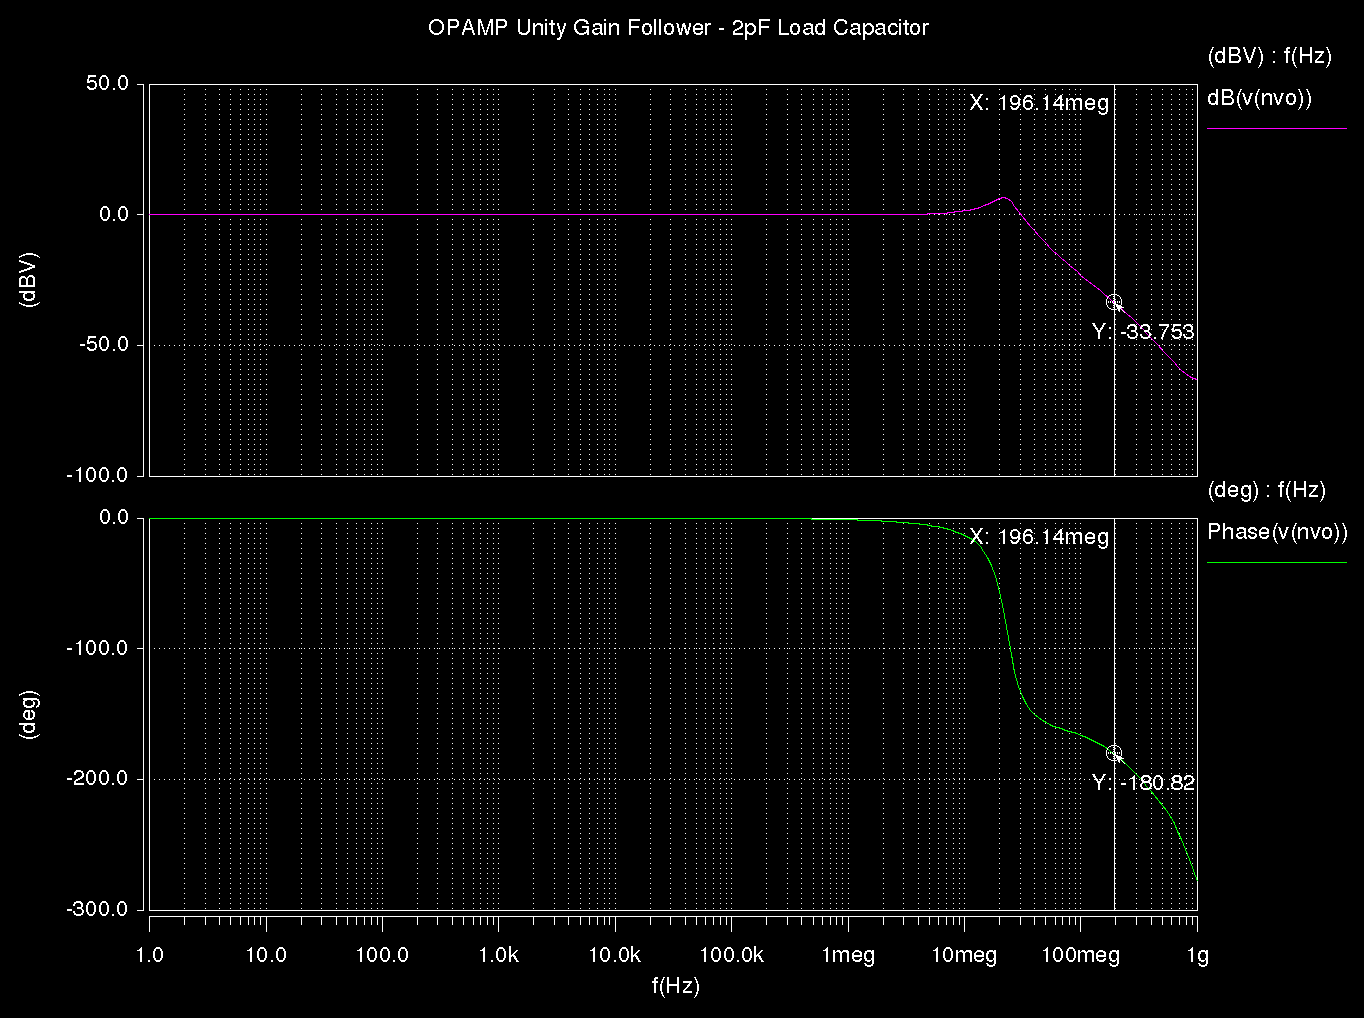
\includegraphics[scale=0.35]{./2pf.png}
\end{center}
\end{figure}
\begin{figure}[h!] 
\begin{center}
 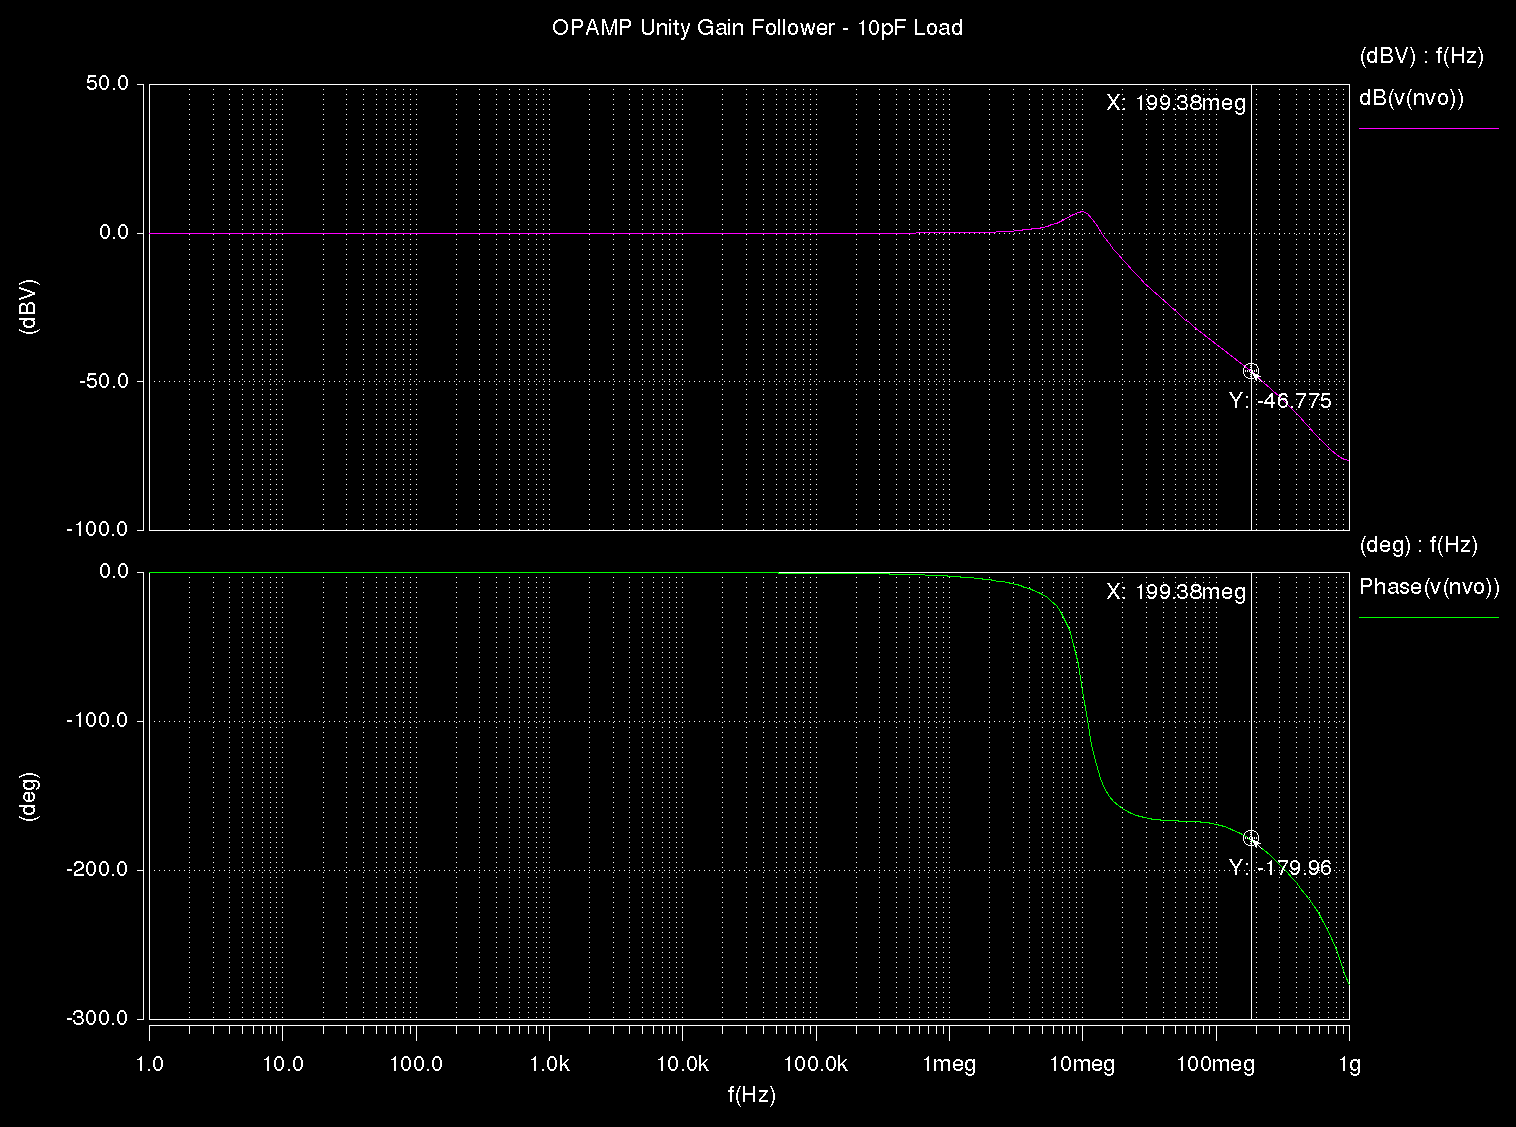
\includegraphics[scale=0.3]{./10p.png}
\end{center}
\end{figure}
\FloatBarrier
\end{document}
